\documentclass [a4paper, 11pt] {article}

%document configuration
\newcommand{\courseName}{Machine Learning in Graphics \& Vision}
\newcommand{\termYear}{Summer Term 2020}
\newcommand{\homeworkNum}{2}
\newcommand{\studentOne}{Driton Goxhufi}
\newcommand{\studentTwo} {Damir Ravlija}
\newcommand{\matrikelNrStOne}{4233242}
\newcommand{\matrikelNrStTwo}{5503184}
\newcommand{\mailStOne}{driton.goxhufi@student.uni-tuebingen.de}
\newcommand{\mailStTwo}{damir.ravlija@student.uni-tuebingen.de}

%packages
\usepackage [english] {babel}
\usepackage [T1] {fontenc}
\usepackage [utf8] {inputenc}
\usepackage {graphicx}
\usepackage {subcaption}
\usepackage {amsmath}
\usepackage {amssymb}
\usepackage {amstext}
\usepackage {amsthm}
\usepackage {listings}
\usepackage {tikz}
\usepackage[
pdftex,
pdfauthor={Goxhufi, Driton; Ravlija, Damir},
pdftitle={MLGV - Exercise \homeworkNum Submission},
pdfsubject={Machine Learning in Graphics \& Vision Homework}
]{hyperref}

\usepackage[a4paper,lmargin={2cm},rmargin={2cm},tmargin={3.5cm},bmargin = {2.5cm},headheight = {4cm}]{geometry}

\usepackage[shortlabels]{enumitem}
\usepackage{lastpage}
\usepackage{fancyhdr}

\usepackage{lipsum}
\usepackage{ifthen}

\pagestyle{fancy}



%other config
\renewcommand{\v}[1]{\boldsymbol{#1}}
\newcommand{\mat}[1]{\boldsymbol{#1}}
\newcommand{\m}[1]{\begin{pmatrix}#1\end{pmatrix}}
\newcommand{\tr}[2]{{}^{#1}T_{#2}}
\graphicspath{{./images/}}


\lhead{\begin{tabular}{l}
		\courseName\\
		\termYear \\
		Exercise \homeworkNum
\end{tabular}}
\rhead{\begin{tabular}{lr}
		\studentOne & \matrikelNrStOne \\
		\studentTwo & \matrikelNrStTwo \\
\end{tabular}}

\begin{document}
	
\title{\vspace{-1.5cm}\textbf{Exercise \homeworkNum} \\ 
	\courseName}
\author{\begin{tabular}{lcr}
		\studentOne & \matrikelNrStOne & \href{mailto:\mailStOne}{\mailStOne} \\
		\studentTwo & \matrikelNrStTwo & \href{mailto:\mailStTwo}{\mailStTwo} 
\end{tabular}}	
\date{}
\maketitle


\section{Task 1}
\begin{enumerate}
\item[(a)]
Classification accuracy of the initialized model on the test dataset is $0.5$


\item[(b)]
Loss of the initialized model is $0.7149616252170096$.

\item[(c)]
In the first step of derivation we use the chain rule and the fact that $f_{\v{w}}'(x) = f_{\v{w}}(x)(1-f_{\v{w}}(x)$.
\begin{align*}
\frac{\partial L(\v{x}, t, \v{w})}{\partial \v{w}} &\stackrel{(\ref{eq:c})}{=} \frac{1}{N}\sum_{n=1}^{N}\left[-t_n \frac{1}{f_{\v{w}}(\v{x}_n)}f_{\v{w}}(\v{x}_n)(1-f_{\v{w}}(\v{x}_n))\v{x}_n + (1-t_n)\frac{1}{1-f_{\v{w}}(\v{x_n})}f_{\v{w}}(\v{x}_n)(1-f_{\v{w}}(\v{x}_n))\v{x}_n \right] \\
&= \frac{1}{N}\sum_{n=1}^{N}\left[-t_n(1-f_{\v{w}}(\v{x}_n))\v{x}_n + (1-t_n)f_{\v{w}}(\v{x}_n)\v{x}_n \right] \\
&= \frac{1}{N}\sum_{n=1}^{N}\left[(-t_n + t_n f_{\v{w}}(\v{x}_n) + f_{\v{w}}(\v{x}_n) - t_nf_{\v{w}}(\v{x}_n))\v{x}_n\right] \\
&= \frac{1}{N}\sum_{n=1}^{N}\left[ f_{\v{w}}(\v{x}_n) - t_n\right]\v{x}_n
\end{align*}

\begin{enumerate}
	\item[(1)]\label{eq:c} 
	\begin{align*}
	\frac{\partial f_{\v{w}}(x)}{\partial x} &= \frac{\partial}{\partial x}\left(\frac{1}{1 + e^{-\v{w}^{T}\v{x}}}\right) = \frac{e^{-\v{w}^{T}\v{x}}}{{(1 + e^{-\v{w}^{T}\v{x}})}^2} = \frac{1 + e^{-\v{w}^{T}\v{x}} - 1}{{(1 + e^{-\v{w}^{T}\v{x}})}^2} = \frac{1}{{(1 + e^{-\v{w}^{T}\v{x}})}} - \frac{1}{{(1 + e^{-\v{w}^{T}\v{x}})}^2} \\
	&= \frac{1}{{(1 + e^{-\v{w}^{T}\v{x}})}} \left(1 - \frac{1}{{(1 + e^{-\v{w}^{T}\v{x}})}}\right) = f_{\v{w}}(\v{w}^{T}\v{x})(1 - f_{\v{w}}(\v{w}^{T}\v{x}))
	\end{align*}
\end{enumerate}

\bigskip
\bigskip
\bigskip

After $1,000$ iterations the loss and accuracy of the model are:

	\qquad loss $= 0.3868595564299156$
	
	\qquad accuracy $= 0.83$



	
\item[(d)]
\begin{figure}[!h]
	\centering
	\begin{subfigure}{0.4\textwidth}
		\centering
		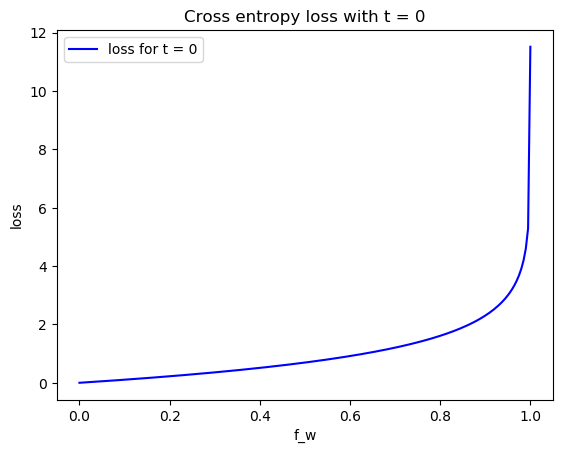
\includegraphics[width=\textwidth]{img/2_1_d_1.png}
		\caption{With loss $t = 0$}
		\label{fig:1a}
	\end{subfigure}
	\begin{subfigure}{0.4\textwidth}
		\centering
		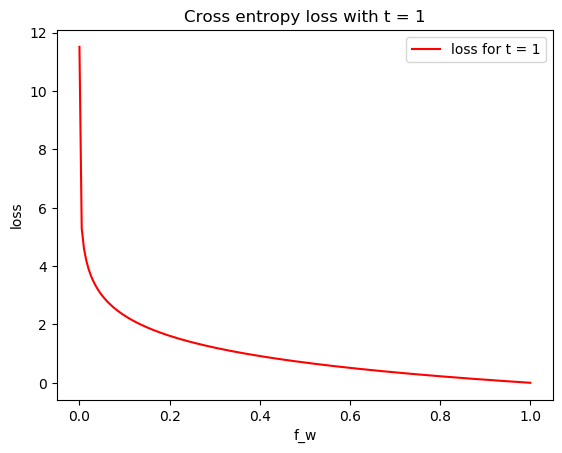
\includegraphics[width=\textwidth]{img/2_1_d_2.png}
		\caption{With loss $t = 1$}
		\label{fig:1b}
	\end{subfigure}
	\caption{Plot of results from task (d)}
	\label{fig:1}
\end{figure}

\end{enumerate}
	
\end{document}

